22. \begin{figure}[ht!]
\center{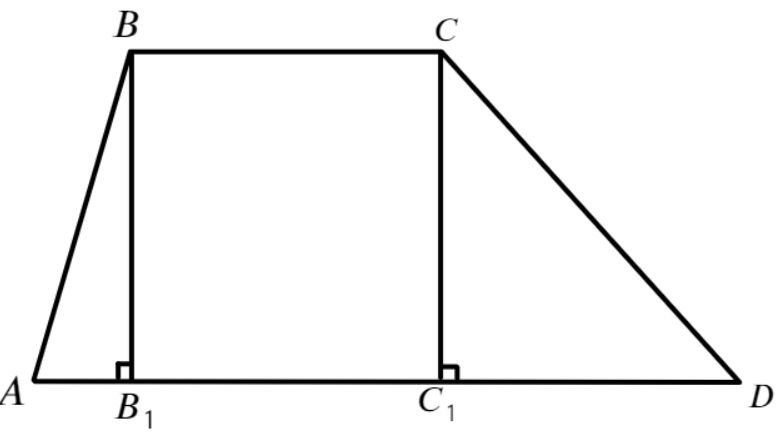
\includegraphics[scale=0.35]{g9-21.png}}
\end{figure}\\
Опустим высоты $BB_1$ и $CC_1.$ Пусть $AB=5$см, $BC=6$см, $CD=12$см, $AD=7$см, $AB_1=x.$ Тогда $C_1D=7-6-x=1-x$ и по теореме Пифагора имеем равенства
$5^2-x^2=BB_1^2=CC_1^2=12^2-(1-x)^2,\ 25-x^2=144-1+2x-x^2,\ 2x=-118,\ x=-59$. Полученный отрицательный результат говорит о том, что на самом деле картинка выглядит по-другому и высота из точки $B$ падает на продолжение основания $AD.$
ewpage
oindent
\begin{figure}[ht!]
\center{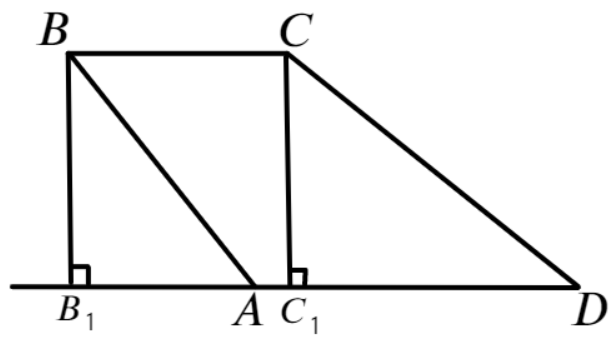
\includegraphics[scale=0.35]{g9-21-1.png}}
\end{figure}\\
Тогда если $AB_1=x,$ то $AC_1=6-x,\ C_1D=7-(6-x)=x+1$ и $5^2-x^2=BB_1^2=CC_1^2=12^2-(x+1)^2,\ 25-x^2=144-1-2x-x^2,\ 2x=118,\ x=59$см. Но тогда в треугольнике
$ABB_1$ катет длиннее гипотенузы, что невозможно, значит такой трапеции не существует.\\
